\section{ Object Recognition }
\subsection{Functional Requirements}
	\begin{flushleft}
		\begin{itemize}
			\item{\textbf{R3:}} FMDS will \textbf{detect objects} in the reserve
				\begin{itemize}
					\item{\textbf{R3.1}} FMDS will allow the ranger to see a list of \textbf{objects} and their \textbf{locations}.
					\item{\textbf{R3.2}} FMDS will draw a rectangle around the objects that it detects.
					\item{\textbf{R3.2}} FMDS will notify the ranger of the objects that it detects.
				\end{itemize}
		\end{itemize}
	\end{flushleft}

\subsection{Use Case Diagram}
\begin{flushleft}
	\begin{figure}[h!]
		\centering
		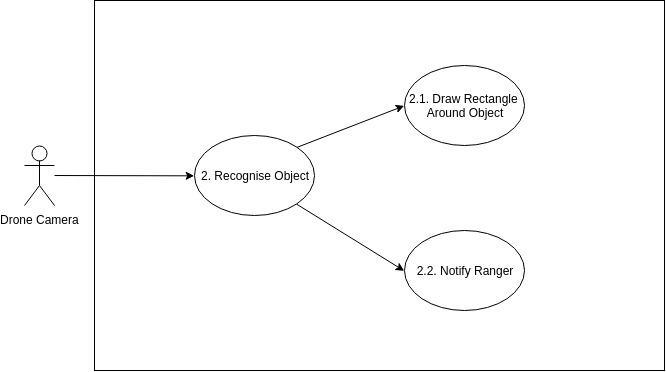
\includegraphics[scale=0.5]{./assets/images/object-recognition-ucd.jpg}
		\label{fig: object-recognition-ucd }
		\caption{Object Recognition Use Case Diagram}
	\end{figure}

\end{flushleft}

